%%%% CAPÍTULO 4 - RESULTADOS E DISCUSSÃO

\chapter{RESULTADOS E DISCUSSÃO}\label{cap:resultados}

Para alcançar resultados ainda mais satisfatórios, especialmente no que diz respeito 
ao processo de identificação e reconhecimento facial, seriam necessários recursos 
de processamento de imagem adicionais para o ESP32. Apesar de o \textit{chip} ESP32 
apresentar considerável poder de processamento, ele nem sempre oferece recursos 
de \textit{hardware} suficientes para tarefas intensivas de processamento de 
imagem e visão computacional. Como resultado, a maioria das bibliotecas de 
visão computacional e seus métodos não estão disponíveis para o ESP32.

No entanto, é possível realizar processamento de imagem básico e funções 
relacionadas à detecção e reconhecimento facial no ESP32, devido a 
otimizações de código de aprendizado profundo (ESP-DL) e implementações 
específicas voltadas para dispositivos com menor capacidade de processamento.

Para uma comparação qualitativa dos resultados atuais com outras implementações, 
a disponibilidade de bibliotecas de visão computacional, como o OpenCV, 
seria altamente benéfica. Embora as bibliotecas oficiais sejam limitadas, 
é possível encontrar bibliotecas não oficiais desenvolvidas por colaboradores 
que possuem métodos de processamento de imagem inspirados nas bibliotecas 
já existentes. Avaliar a influência da luminosidade nas imagens e a eficácia 
de parâmetros ou funções específicas é importante para combinar métodos 
alternativos visando obter melhores resultados.

Na \autoref{fig:espgrayopencv}, é possível observar as imagens com níveis 
de luminosidade diferentes. O cenário ideal seria que, independentemente 
da iluminação estar alta ou baixa, o resultado do processo de reconhecimento 
fosse igualmente eficaz, assemelhando-se ao desempenho em condições 
ideais de luminosidade. No entanto, 
é fundamental considerar que outros tipos de erros 
ainda podem ocorrer.

\begin{figure}[h!]
    \centering
    \caption{Transformações monótonas em escala de cinza}
    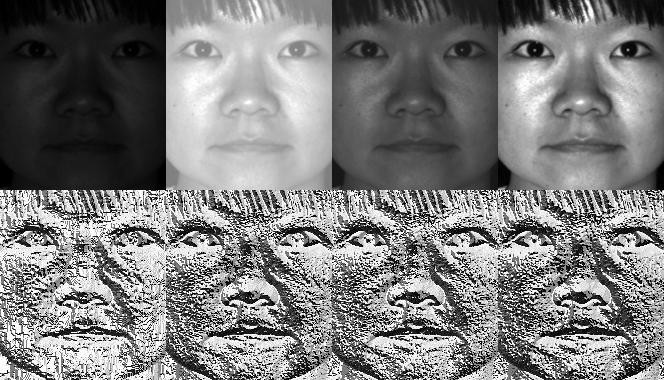
\includegraphics[scale=0.5]{figuras/escala_cinza.jpg} 
    \legend{Fonte: Adaptado de \citeonline{opencv3}.}
    \label{fig:espgrayopencv}
    \centering
\end{figure}

O protótipo atual satisfaz praticamente todas as necessidades do projeto, 
como detecção e reconhecimento facial, cadastro de usuários e implementação 
do temporizador. Portanto, atende aos requisitos estabelecidos durante 
o desenvolvimento.

No entanto, há espaço para melhorias a curto e longo prazo. Isso inclui 
atualizações contínuas, como a possibilidade de configurar o número de 
usuários cadastrados, a exibição de IDs de usuários e a adição de 
métodos para excluir usuários por ID. Além disso, a funcionalidade 
de permitir que um usuário administrador altere senhas de cadastro 
e a de remover todos os usuários.

Outra melhoria relevante seria a integração do protótipo em aplicativos 
e servidores da web, ampliando suas possibilidades de aplicação prática, 
como em sistemas de controle de acesso residencial ou empresarial 
totalmente baseados na web.

Por último, uma melhoria significativa envolveria a criação de uma 
placa personalizada, partindo do zero, usando inicialmente apenas o \textit{chip} 
ESP32. Isso permitiria a liberação do I2C para uso geral, 
possibilitando a integração de novos recursos devido ao aumento 
da quantidade de portas (GPIO) disponíveis.